\chapter{Validating graphs}\label{sec:valGraph}

In the previous section, we described an algorithm to verify proof trees. Proofs trees are a very natural way to encode certificates for datalog results but have some drawbacks. 

\begin{example}\label{ex:treeGraph}
    Consider the following program that computes the transitive closure. We double an atom in the body which does not change the semantics of the rule. 

    \begin{align}
            T(?x,?y) &\leftarrow E(?x,?y). \label{ex:treeGraph:ruleBase}\\
            T(?x,?z) &\leftarrow T(?x, ?y), T(?x, ?y), E(?y, ?z). \label{ex:treeGraph:ruleTrans}
    \end{align}

    The database shall encode the elements of a chain $E(i, i+1)$ for $i \in \{0, n\}$. In the proof tree representation, we need the same proof tree twice for $T(?y, ?z)$ in the second rule and will need copies for it later, which results in large trees. The proof tree for $T(0, i+1)$ needs a vertex representing the head of \cref{ex:treeGraph:ruleTrans}, one vertex for the $E$ fact $E(i, i+1)$ and two proof trees for $T(0, i)$. Therefore the size of $T(0, i+1)$ in the number of nodes is more than double the size of $T(0, i)$ which leads to an exponential growth.
\end{example}

Proof trees offer no reusability of atoms as they need to stay in the tree shape. If an atom is used multiple times in the derivation we need for each usage a new vertex that is labeled by this atom. Formally we can view the proof tree as a directed tree $T= (V_T;E_T)$ with a label function $label: V_T \to groundAtom$ because different vertices can have the same label in a proof tree as in the example above. We need this as a ground atom $a$ can be used in multiple ground rules in the derivation but cannot have connections from multiple vertices to the vertex representing $a$ if we are in a directed tree.

A more compact representation would be a directed graph $G=(V_G, E_G)$ of $T$  with $V_G = \{a \mid \exists v \in V_T, label(v)=a\}$ and $E_G = \{ (a_1, a_2) \mid \exists v_1, v_2 \in V_T,  label(v_i) = a_i \land (v_1, v_2) \in E_T\}$. Then a vertice can be considered equal to its label as no label occurs multiple times anymore. Examples of a proof tree and the corresponding graph are in \cref{fig:treeGraph}.


\begin{figure}
  \centering
  \begin{subfigure}[b]{0.5\textwidth}
    \centering
    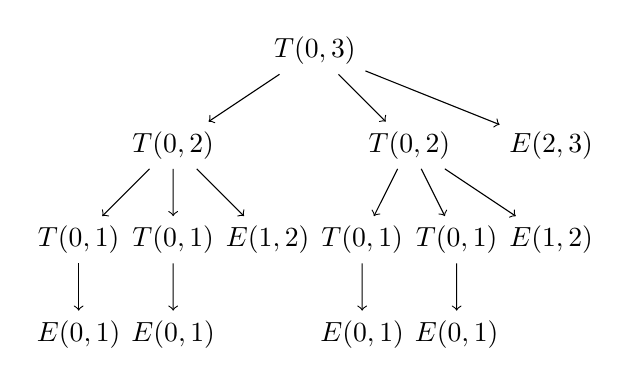
\begin{tikzpicture}[scale=.6]
      \node (A) at (5,4) {$T(0,3)$};

      \node (B) at (2,2) {$T(0,2)$};
      \node (C) at (7,2) {$T(0,2)$};
      \node (D) at (10,2) {$E(2,3)$};

      \node (E) at (0,0) {$T(0,1)$};
      \node (F) at (2,0) {$T(0,1)$};
      \node (G) at (4,0) {$E(1,2)$};
      \node (H) at (6,0) {$T(0,1)$};
      \node (I) at (8,0) {$T(0,1)$};
      \node (J) at (10,0) {$E(1,2)$};

      \node (K) at (0,-2) {$E(0,1)$};
      \node (L) at (2,-2) {$E(0,1)$};
      \node (M) at (6,-2) {$E(0,1)$};
      \node (N) at (8,-2) {$E(0,1)$};

      \draw[->] (A) -- (B);
      \draw[->] (A) -- (C);
      \draw[->] (A) -- (D);
      \draw[->] (B) -- (E);
      \draw[->] (B) -- (F);
      \draw[->] (B) -- (G);
      \draw[->] (C) -- (H);
      \draw[->] (C) -- (I);
      \draw[->] (C) -- (J);
      \draw[->] (E) -- (K);
      \draw[->] (F) -- (L);
      \draw[->] (H) -- (M);
      \draw[->] (I) -- (N);
    \end{tikzpicture}
    \caption{A proof tree for $T(0,3)$}
    \label{fig:proofTree}
  \end{subfigure}
  \hfill
  \begin{subfigure}[b]{0.4\textwidth}
    \begin{tikzpicture}[scale=0.9]
      \node[circle] (A) at (0,4) {$T(0,3)$};
      \node[circle] (B) at (-1,2) {$T(0,2)$};
      \node[circle] (C) at (2,2) {$E(2,3)$};
      \node[circle] (D) at (-1,0) {$T(0,1)$};
      \node[circle] (E) at (2,0) {$E(1,2)$};
      \node[circle] (F) at (-1,-2) {$E(0,1)$};

      \draw [->] (A) -- (C);
      \draw[->] (A) to[out=235, in=150] (B);
      \draw[->] (A) to[out=280, in=45] (B);
      \draw [->] (B) -- (E);
      \draw[->] (B) to[out=235, in=150] (D);
      \draw[->] (B) to[out=280, in=45] (D);
      \draw[->] (D) -- (F);
    \end{tikzpicture}
    \caption{A proof graph for $T(0,3)$}
    \label{fig:proofGraph}
  \end{subfigure}
  \caption{An example of a proof tree and a proof graph for the same fact from \cref{ex:treeGraph}}
  \label{fig:treeGraph}
\end{figure}

Another advantage occurs when we want to validate multiple trees or even a complete result. Multiple trees will often share labels as well and combining them into a graph, i.e. the union of $G_{T_i}$ for trees $T_i$ will again include every label just once. In the previous section, we introduced the possibility of not having to check every proof tree as they occur in other proof trees as well. Selecting a minimal amount of proof trees to check a complete result is however still an instance of the NP-hard subset cover problem.

We require for this that the successors of a ground atom are the same elements in every tree if the ground atom occurred in this tree. If not an atom would have more successors in the graph than previously in the trees and there will probably exist no matching ground rule. In practice, this requirement was always fulfilled.

Another requirement is acyclicity. We cannot use an atom to explain itself. Either we could have used it directly before or it cannot be explained by a proof tree at all. 
\section{Graph model}

As a number of different results from mathematics are already formalized in Mathlib, it is no surprise that graphs are already modeled in Mathlib as depicted below:

\begin{lstlisting}
structure SimpleGraph (V : Type u) where
  /-- The adjacency relation of a simple graph. -/
  Adj : V → V → Prop
  symm : Symmetric Adj 
  loopless : Irreflexive Adj
\end{lstlisting}

This graph representation is unfortunately not what we need in an algorithm. Firstly, the adjacency relation of this graph is always symmetric so it does not encode the directed graphs we need. The direction of the edges allows us to differentiate between the ground atoms that were used to derive a ground atom and the ground atoms that were derived from a ground atom. Secondly, the adjacency relation is a function to \lstinline|Prop| and thus in general not computable but we want to use it in an algorithm. Finally, we need the successors of a vertex to verify the vertex as they are supposed to represent the body of a ground rule. When we want to obtain the successors in this graph model we would have to query the adjacency relation for every vertex assuming it would be computable.

Therefore we design our own implementation of a graph. We use an adjacency list approach so that we can quickly get all the successors of a vertex. The graph is represented by a hash map whose keys are the vertices. Each vertex is mapped via the hash map towards its successors.

\begin{lstlisting}
    abbrev (.\PreGraph.) (A: Type) [DecidableEq A] [Hashable A] := 
        Std.HashMap A (List A)

    def (.\PreGraphvertices.) (g : PreGraph A) : List A := g.toList.map Prod.fst
    def (.\PreGraphsuccessors.) (g : PreGraph A) (a : A) : List A := g.findD a []
\end{lstlisting}

\lstinline|Std.HashMap.toList| returns here a list of pairs of the type $(A, List\ A)$, i.e. a vertex and its successors. Using \lstinline|Prod.fst| we obtain the first element of every pair in the list, which are all vertices. \lstinline|Std.HashMap.findD a []| returns the value saved with $a$ in the hash map which are the successors of $a$. If a vertex is not present (the key is not in the hash map), then $[]$ is returned which is the fallback option provided to  \lstinline|Std.HashMap.findD|.

This approach contains all important elements in a graph, but there is a small technical problem with it. 

\begin{example}\label{ex:incompletePregraph}
    
    Consider the graph depicted in \cref{ex:counterexampleGraph}. An element is colored, if it is in the list of vertices. Hence, the vertices are the list $[1,2,3]$. The vertex 3 has the element 4 as a successor, but 4 is not a vertex of the graph. Such a behavior is undesirable as searching for vertices that satisfy some criteria may lead outside of the graph.

\begin{figure}
    \centering
    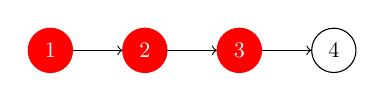
\begin{tikzpicture}[scale=0.8,transform shape]
        % Define styles for nodes and edges
        \tikzstyle{vertex}=[circle, draw=black, fill=white, minimum size=20pt, inner sep=0pt]
        \tikzstyle{rednode}=[vertex, red]
      
        % Define vertices
        \node[rednode] (v1) at (1.5,0) {\textcolor{white}{1}};
        \node[rednode] (v2) at (3,0) {\textcolor{white}{2}};
        \node[rednode] (v3) at (4.5,0) {\textcolor{white}{3}};
        \node[vertex] (v4) at (6,0) {4};
      
        % Draw edges
        \draw[->] (v1) -- (v2);
        \draw[->] (v2) -- (v3);
        \draw[->] (v3) -- (v4);
      
      \end{tikzpicture}
    \caption{An example of an incomplete pregraph for \cref{ex:incompletePregraph}}      
    \label{ex:counterexampleGraph}

\end{figure}
    
\end{example}

We define a pregraph to be complete if every successor of a vertex is a vertex itself and thus can avoid the problem.

\begin{lstlisting}
    def (.\PreGraphcomplete.) (pg: PreGraph A) := 
    ∀ (a:A), pg.contains a →  ∀ (a':A), a' ∈ (pg.successors a) → pg.contains a'
\end{lstlisting}

A graph is then a complete pre-graph and we can lift all previous operations to this new type.
\begin{lstlisting}
abbrev (.\Graph.) (A: Type) [DecidableEq A] [Hashable A] := 
    { pg : PreGraph A // pg.complete }
\end{lstlisting}

The completeness predicate was necessary because not all elements of the type $A$ are vertices but the successors of a vertex can be any element of the type $A$.
We start by formalizing walks in a graph. Walks allow the repetition of vertices in itself in contrast to paths which suffices our needs. 

A walk $w$ in a graph $G$ is a list of vertices that are all vertices of $G$ and are connected via the successor relation of $G$, i.e. for every $i$ with $0 < i < i.length$ we have that $w[i-1] \in G.successors\ w[i]$. The starting vertex of the walk is consequently at the back.

\begin{lstlisting}
def (.\isWalk.) (l: List A) (G: Graph A): Prop :=
    (∀ (a:A), a ∈ l → a ∈ G.vertices ) ∧ 
    ∀ (i: ℕ), i > 0 → ∀ (g: i < l.length), l.get (Fin.mk i.pred (pred_lt i l.length g)) ∈ G.successors (l.get (Fin.mk i g) )
\end{lstlisting}

The \lstinline|pred| function returns the predecessor of any natural number that is not zero and zero otherwise. Because we use the \lstinline|List.get| function we not only have to specify a position but also a proof that this position is smaller than the length of the list to not get an error. These two elements are combined into a Fin type. In the future, we usually omit these proofs in this work because of the length. The proofs can however be found in the actual formalization.

Due to the completeness predicate it would suffice to require that the starting vertex is in $G$ but this variant is simpler to state. We also allow the empty walk $[]$ as this will be beneficial in later applications.

Lists are better in this use case in contrast to arrays because they can easily be extended at the front which we will use when exploring a graph algorithmically. We can always extend a walk by a successor of the leading element.

\begin{lemma}[\isWalkextendssuccessors]
    Let $w$ be a list of vertices and $a$ and $b$ be vertices.
    If $a::w$ is a walk in $G$ and $b$ is a successor of $a$ in G then $b::a::w$ is also a walk in $G$.
\end{lemma}

A cycle is supposed to be a walk that starts and ends with the same node and an acyclic graph is a graph that has no cycles. Any list that only contains a single vertex of the graph would consequently be a cycle. Hence, we require that a cycle has additionally at a minimal length of two.

\begin{lstlisting}
def (.\isCycle.) (l: List A) (G: Graph A): Prop :=
  if h: l.length < 2
  then False
  else

  isWalk l G ∧ l.get (Fin.mk 0 _) = l.get (Fin.mk l.length.pred _)

def (.\isAcyclic.) (G: Graph A) := ∀ (l: List A), ¬ isCycle l G
\end{lstlisting}

\section{Validation of a graph}

After defining the graph model, we want to specify how the graph validation takes place. For trees, we defined the recursive predicate \isValid and implemented it using \treeValidator. As the graph we receive may not even be acyclic we cannot simply define a recursive predicate as this will then not terminate. Instead, we define a local predicate for each vertex and its successor. Then we can check every vertex individually.

\begin{lstlisting}
def (.\locallyValid.) (P: program τ) (d: database τ) (v: groundAtom τ) (G: Graph (groundAtom τ)): Prop :=
 (∃(r: rule τ) (g:grounding τ), r ∈ P 
    ∧ ruleGrounding r g = {head:= v, body:= (G.successors v) }) 
 ∨ ((G.successors v) = [] ∧ d.contains v)
\end{lstlisting}

Except for the rule case, this is very similar to \isValid. Therefore we can reuse earlier concepts and build a checker for this. We expect the program again parsed into a look-up structure $m$, a database $d$, the vertex $a$ and its successors passed as a list $l$.

\begin{lstlisting}
def (.\localValidityCheck.) (m: List τ.relationSymbols → List (rule τ)) (d: database τ) (l: List (groundAtom τ)) (a: groundAtom τ) : Except String Unit :=
  if l.isEmpty
  then
    if d.contains a
    then Except.ok ()
    else checkRuleMatch m (groundRule.mk a l)
  else
    checkRuleMatch m (groundRule.mk a l)
\end{lstlisting}

The correctness is proven similar to before assuming that $m$ is the result of \parseProgramToSymbolSequenceMap of the program $P$.

\begin{lemma}[\localValidityCheckUnitIffLocallyValid]
    Let $d$ be a database and $P$ be a program. If $m$ is the result of \parseProgramToSymbolSequenceMap with a function that maps any element to the empty list and $l$ is the list of successors of a ground atom $a$. Then the \localValidityCheck returns ok iff $a$ is locally valid with respect to $P$ and $d$.
\end{lemma}

In the next section, we will show a method to show that a graph is acyclic and all vertices are locally valid with respect to $P$ and $d$. In the remainder of this section, we assume that this is true and devise a method to show that then all vertices of the graph are in the proof-theoretic semantics of $P$ and $d$.

Our goal is to create a valid proof tree for every vertex. We devise a function that creates such a proof tree for a given vertex by recursively calling it on the successors.

\begin{lstlisting}
def (.\extractTree.) (a: A) (G: Graph A) (mem: a ∈ G.vertices) (acyclic: isAcyclic G): tree A :=
  tree.node a (List.map (fun ⟨x, _h⟩ => extractTree x G (G.complete a mem x _h) acyclic) (G.successors a).attach)
\end{lstlisting}

This function only terminates because the graph is acyclic. Therefore we require the acyclicity as an explicit argument in the function. We will show the termination by using the number of vertices that are reachable from the current vertex. These decrease the further we walk in the graph or else we would be able to reach a previous node and have a cycle which is not allowed. We start by formalizing the notion of reachability. We say that a vertex $a$ \canReach a vertex $b$ if there exists a walk $w$ from $a$ to $b$. (The start of the walk is the last element in the list).

\begin{lstlisting}
    def (.\canReach.) (a b: A) (G: Graph A):= 
    ∃ (p: List A) (neq: p ≠ []), 
        isWalk p G ∧ p.get (Fin.mk 0 _) = b 
        ∧ p.get (Fin.mk p.length.pred _) = a
\end{lstlisting}

Any vertex $a$ can reach itself via the walk $[a]$(\canReachrefl).

We want to use the finite set of the vertices that are reachable from the current node so that we can argue that the cardinality of this set decreases and by this, the function terminates. This set will be a subset of the vertices of the graph $G$ since any element reachable by a walk in $G$ must be in the vertices of $G$. Ideally, we want to filter this finite set to only keep those vertices reachable from the current node. Unfortunately, \lstinline|Finset.filter| requires a decidable predicate. This predicate is in principle decidable for example by Dijkstra's algorithm. Instead of implementing and validating it, we instead use classical logic to obtain that any predicate is decidable and reuse the previous filter version. This is now no longer computable but we only want to use it in the termination proof anyway.

\begin{lstlisting}
noncomputable def (.\Finsetfilternc.) (p: A → Prop) (S: Finset A):= @Finset.filter A p (Classical.decPred p) S

lemma (.\Finsetmemfilternc.) (a:A) (p: A → Prop) (S: Finset A): a ∈ Finset.filter_nc p S ↔ p a ∧ a ∈ S
\end{lstlisting}

The global successors in a graph $G$ of a vertex $a$ are then all the vertices $b$ that are reachable from $a$ in $G$.

\begin{lstlisting}
    noncomputable def (.\globalSuccessors.) (a:A) (G: Graph A): Finset A := Finset.filter_nc (fun b => canReach a b G) G.vertices.toFinset
\end{lstlisting}

\begin{figure}
    \centering
    \begin{tikzpicture}[every node/.style={circle,draw},level 1/.style={sibling distance=40mm},level 2/.style={sibling distance=20mm},level 3/.style={sibling distance=10mm}]
        \node {1}
          child {node[fill=blue!30] {2}
            child {node[diagonal fill={red!30}{blue!30}] {4}
              child {node[diagonal fill={red!30}{blue!30}] {8}}
              child {node[diagonal fill={red!30}{blue!30}] {9}}
            }
            child {node[fill=blue!30] {5}
              child {node[fill=blue!30] {10}}
              child {node[fill=blue!30] {11}}
            }
          }
          child {node {3}
            child {node {6}
              child {node {12}}
              child {node {13}}
            }
            child {node {7}
              child {node {14}}
              child {node {15}}
            }
          };
      \end{tikzpicture}
      \caption{The global successors of $2$ are colored blue, the global successors of $4$ are colored red.}
      \label{fig:globalSuccessors}
\end{figure}

We already see in \cref{fig:globalSuccessors} that the global successors of $2$ are a strict subset of the global successors of $4$ and $4$ is the successor of $2$. We can generalize this. In any graph we have that for every vertex $a$ and successor $b$ of $a$ we have that $globalSuccessors(b) \subseteq globalSuccessors(a)$, because any element $c$ that $b$ can reach can also be reached from $a$ by first going to $b$ and then following the walk from $b$ to $c$

(\globalSuccessorsSubsetWhenSuccessor).


If the graph is additionally acyclic, we get that $globalSuccessors(b) \subset globalSuccessors(a)$, because $a$ can reach $b$ via the successor edge. If $b$ could reach $a$, then this would lead to a cycle which is not allowed.

(\globalSuccessorsSSubsetWhenAcyclicAndSuccessor)

Since we call \extractTree on all successors $b$ of $a$ and the global successors of $b$ are a strict subset of the global successors of $a$ the cardinality of the global successors of the vertex we call the function on always decreases.

\begin{lstlisting}
def (.\extractTree.) (a: A) (G: Graph A) (mem: a ∈ G.vertices) (acyclic: isAcyclic G): tree A :=
  tree.node a (List.map (fun ⟨x, _h⟩ => extractTree x G (G.complete a mem x _h) acyclic) (G.successors a).attach)
termination_by Finset.card (globalSuccessors a G)
decreasing_by
  simp_wf
  apply Finset.card_lt_card
  apply globalSuccessorsSSubsetWhenAcyclicAndSuccessor
  apply acyclic
  apply _h
  apply mem
\end{lstlisting}

We see from the definition that the root of the tree returned by extractTree is always the vertex $a$ used in the arguments. (\rootOfExtractTree)

It remains to be shown this leads to a valid proof tree.

\begin{lemma}[\extractTreeValidIffAllLocallyValidAndAcyclic]
    Let $G$ be an acyclic graph where all vertices are locally valid with respect to a program $P$ and database $d$. Then extractTree results in a valid proof tree for any vertex $a$ of $G$.
\end{lemma}
\begin{proof}
    We prove this by strong induction on the cardinality of the global successors of $a$.

    Since $a$ is a vertex of $G$, $a$ is locally valid. There are two cases for this. If $a$ is locally valid because it has no successors and is in the database, then the map operation creates no subtrees so that the resulting proof tree is valid as well.

    If $a$ is locally valid because $a$ and its successors form a ground rule from the ground program of $P$, then we create the subtrees with extractTree. By the previous observation, the roots of the subtrees equal the successors of $a$, so that we have again a ground rule from the ground program. The global successors of any successor of $a$ are a subset of the global successors of $a$ and thus their cardinalities are smaller. Therefore we can apply the induction hypothesis and see that all these trees are then valid as well, so that the proof tree for $a$ is valid.
\end{proof}

Using this result the vertices of an acyclic graph whose vertices are all locally valid with respect to $P$ and $d$ are a subset of the proof-theoretic semantics of $P$ and $d$.

\section{Depth-first search}

By the results of the previous result, we know that in order to verify a graph we have to call the \localValidityCheck on every vertex and its successors and determine whether the graph is acyclic. A typical solution to answer the second question is the depth-first search, which we will implement and verify in this section. During the depth-first search, the algorithm has to visit every vertex. With the aim of reducing the number of iterations over the vertex list, we combine this with executing \localValidityCheck on every vertex and its successors.

We generalize this by considering a function \lstinline|f: A → List A → Except String Unit| for a \lstinline|Graph A|. The Except type is again chosen to return an error message to the user in the negative case.

We follow \cite{AlgorithmsBook} when implementing depth-first search and use several helper functions that simplify the proofs. A first function \dfs starts the process on every vertex and the actual exploration of the graph is done in \dfsstep. So that we do not explore vertices multiple times, we store already explored vertices in a finite set. For performance reasons, this is a hash set instead of the finite set from Mathlib.

The function \isOkOrMessage takes an arbitrary exception whose error type is a string and transforms it into an \lstinline|Except String Unit| object to have a similar output type as the \treeValidator. This returns ok iff the original exception was also an ok element(\isOkOrMessageOkIffExceptionIsOk).

We use \foldlexceptset as a variant as the common \textit{foldl} or \textit{reduce} function. It stops and returns the first found exception. If no exception is found it executes the function on the first element with the input set and then calls itself recursively with the resulting sets. We use this to share the set of already explored vertices in further explorations.

\begin{lstlisting}
def (.\isOkOrMessage.) (e: Except String A): Except String Unit :=
    match e with
    | Except.error msg => Except.error msg
    | Except.ok _ => Except.ok ()

def (.\foldlexceptset.) 
(f: A → HashSet B → (Except String (HashSet B))) 
(l: List A) (init: HashSet B): Except String (HashSet B) :=
  match l with
  | [] => Except.ok init
  | hd::tl =>
    match f hd init with
    | Except.error msg => Except.error msg
    | Except.ok S => foldl_except_set f tl S

def (.\dfs.) (G: Graph A) (f: A → List A → Except String Unit) : Except String Unit :=
    isOkOrMessage (foldl_except_set (fun ⟨x,_h⟩ S => dfs_step x G f [] (isWalkSingleton G x _h) (List.not_mem_nil x) S) G.vertices.attach HashSet.empty )
\end{lstlisting}

The main work is done in \dfsstep which we define next. This function takes a variety of arguments:
\begin{enumerate}
    \item an element $a$ that is the vertex we want to start exploring from,
    \item a graph $G$,
    \item a function \lstinline|f: A → List A → Except String Unit| that shall be evaluated on every vertex and its successors,
    \item a list $currWalk$ of nodes that are the walk we used to arrive at $a$ when exploring the graph,
    \item a proof that $a::currWalk$ are indeed a walk in $G$,
    \item a second proof that $a$ is not in $currWalk$ for the termination proof of this function and
    \item a hash set $visited$ of already explored vertices to allow earlier termination.
\end{enumerate}

We start the algorithm by checking if $a$ is already in $visited$. If that is the case, then we have no further exploration to do and return $visited$. If not we check if $f$ raises an error on $a$ and its successors and return any found error. If $f$ returns ok, we check for a cycle by intersecting $a$'s successors with the current walk. If any successor of $a$ occurs in the current walk, we have found a cycle and return this as an error. If we find no cycle, then we recursively call \dfsstep using \foldlexceptset to update the set of visited vertices on every successor. If no error is found during this exploration, we add $a$ using \addElementIfOk to the returned set by \foldlexceptset before returning it.

\begin{lstlisting}
def (.\addElementIfOk.) [Hashable A] (e: Except B (HashSet A)) (a:A): Except B (HashSet A) :=
  match e with
  | Except.ok S => Except.ok (S.insert a)
  | Except.error msg => Except.error msg

def (.\dfsstep.) [Hashable A] (a: A) (G: Graph A) 
(f: A → List A → Except String Unit) (currWalk: List A) 
(walk: isWalk (a::currWalk) G) (not_mem: ¬ (a ∈ currWalk)) 
(visited: HashSet A) : Except String (HashSet A) :=
  if visited.contains a
  then Except.ok visited
  else
    match f a (G.successors a) with
    | Except.error msg => Except.error msg
    | Except.ok _ =>
      if succ_walk: (G.successors a) ∩ (a::currWalk) = []
      then

      addElementIfOk (foldl_except_set (fun ⟨x, _h⟩ S =>
        dfs_step x G f (a::currWalk) 
        (isWalk_extends_successors walk x _h) 
        (not_mem_of_empty_intersection succ_walk x _h) S) 
        (G.successors a).attach visited) a
      else
        Except.error "Cycle detected"
\end{lstlisting}

This procedure terminates because we call \dfsstep only on elements that do not occur on the current walk. Formally, we show that the cardinality of the finite set \lstinline|(List.toFinset G.vertices \ List.toFinset currWalk)| decreases. Since any element of a walk is a vertex, the cardinality of \lstinline|List.toFinset currWalk| is smaller than the cardinality of the set of vertices. In the recursive calls, the walk is instead $a::currWalk$ and since $a$ is not in $currWalk$ the cardinality of \lstinline|List.toFinset a::currWalk| is larger than the cardinality of \lstinline|List.toFinset currWalk|. The graph stays the same and hence the overall cardinality decreases.

The desired theorem describing the behavior of depth-first search is the following:

\begin{theorem}[\dfssemantics]\label{trm:dfssemantics}
    For any graph $G$ and function \lstinline|f: A → List A → Except String Unit|, \dfs $G$ $f$ returns ok iff the graph is acyclic and $f$ is evaluated to ok for every vertex $a$ of $G$ and its successors.
\end{theorem}

We defined acyclicity by stating that no list of elements of type $A$ is a cycle in $G$ but we do not check all lists for being a cycle in $G$. Therefore we need another criteria for acyclicity that works on the vertex level. A first try is the membership in a cycle. A graph is obviously acyclic if no vertex is a member in a cycle. This is however not sufficient as the next example shows.

\begin{figure}
  \center
  \begin{tikzpicture}
    \node (A) at (9,0) {A};
    \node (B) at (6,0) {B};
    \node (C) at (3,0) {C};
    \node (D) at (0,0) {D};

    \draw[->] (B) -- (A);
    \draw[->] (C) -- (B);
    \draw[->] (A) to [out=165,in=15] (C);
    \draw[->] (D) -- (C);

    \node at (0,-0.4) {\scriptsize\textcolor{sortcolor}{D is not in a cycle.}};
    \node at (0,-0.7) {\scriptsize\textcolor{keywordcolor}{D can reach  a cycle.}};

    % \node at (3,-0.4) {\scriptsize\textcolor{keywordcolor}{In Cycle}};
    % \node at (3,-0.7) {\scriptsize\textcolor{keywordcolor}{Reach. from Cycle}};

    \node at (6,-0.4) {\scriptsize\textcolor{keywordcolor}{A,B,C are all in a cycle.}};
    \node at (6,-0.7) {\scriptsize\textcolor{keywordcolor}{A,B,C all can reach  a cycle.}};

    % \node at (9,-0.4) {\scriptsize\textcolor{keywordcolor}{In Cycle}};
    % \node at (9,-0.7) {\scriptsize\textcolor{keywordcolor}{Reach. from Cycle}};
  \end{tikzpicture}
  \caption{Propagating Acyclicity Check Results via Depth-First Search in \cref{ex:propagatingAcyclicityResultinDFS}.}\label{fig:propagatingAcyclicityResultinDFS}
\end{figure}

\begin{example}
  \label{ex:propagatingAcyclicityResultinDFS}
  

  Suppose that we start \dfsstep on the vertex $D$ on the graph depicted in \cref{fig:propagatingAcyclicityResultinDFS}. We will start exploring $D$, then $C$, $B$ and $A$. During the exploration of $A$ we notice that its successor $C$ already occurs in the current walk. Hence, we found a cycle. If we use membership in a cycle, then this information is not propagated back to $D$. \dfsstep returned an error for $D$ while $D$ is not a member in a cycle. Instead, we desire an iff relation between our criterion and the output of \dfsstep. An alternative is the ability to reach a cycle. This is propagated back and a criterion for when \dfsstep returns ok, which we will formalize now.
\end{example}

We reuse the \canReach predicate for the new \reachesCycle predicate. A vertex $a$ reaches a cycle, if there exists a cycle $c$ with a member $b$ that $a$ can reach.

\begin{lstlisting}
  def (.\reachesCycle.) (a:A) (G: Graph A):= 
  ∃ (c: List A), isCycle c G ∧ ∃ (b: A), b ∈ c ∧ canReach a b G
\end{lstlisting}

We see from the definitions that a graph $G$ is acyclic iff every vertex in $G$ does not reach a cycle. 


\begin{lemma}[\acyclicIffAllNotReachCycle]\label{lem:acyclicIffAllNotReachCycle}
  A graph $G$ is acyclic iff all vertices of $G$ do not reach a cycle.
\end{lemma}
\begin{proof}
  If $G$ is acyclic, then showing that all vertices of $G$ are not reached from a cycle is equivalent to showing that any cycle in $G$ cannot reach any element. Due to the acyclicity, we know that no cycles exist in G so the first direction is shown.

  The back direction is proved via contradiction. Assuming that the graph is not acyclic, we know that there must exist a cycle $c$ in $G$. Cycles in $G$ are nonempty lists of vertices that are all in $G$. As any vertex can reach itself, there is a vertex reached from a cycle in contrast to our assumption, so we have reached the contradiction.
\end{proof}

This property is propagated back from the successors.

\begin{lemma}[\NotreachesCycleIffSuccessorsNotReachCycle]
  A vertex $a$ does not reach a cycle iff every successor of $a$ does not reach a cycle.
\end{lemma}
\begin{proof}
  Both directions are proven via the contraposition. For the forward direction, we have that there is a successor $b$ of $a$ that reaches a cycle. Then we can simply extend the walk by adding $a$ at the back and then $a$ can reach a cycle.

  For the backward direction, we assume that $a$ reaches a cycle by a walk $w$ and try to show that one of its successors must also be able to reach a cycle. 
  If $a$ reaches a cycle $c$ with an element $b$ we consider two cases. 
  If $b$ would be a successor of $a$, we have shown our goal.
  
  Now we assume that $b$ is not a successor of $a$. Again we can consider two cases. If the walk $w$ is of length one then $a$ and $b$ must be equal and $a$ is a member in a cycle itself. As long as $a$ is not the first element in the cycle, we can simply pick the preceding element in the cycle due to the connectedness property of the walk. This does not work if $a$ is the first element of the cycle, but since it is a cycle $a$ must also be the last element and we can pick the predecessor of the last element, which is a successor of $a$ and in a cycle.

  If $a$ reaches $b$ with a walk $w$ longer than length 1, then the walk $w$ must have at least three elements since $b$ is not a successor of $a$. Therefore the walk must have the form $b, \dots ,p, a$ for a successor $p$ of $a$. Then also $p$ reaches a cycle.
\end{proof}

We detect a cycle if a successor $b$ of the current vertex $a$ already occurs in the current walk or if it is equal to $a$. This tells us that we can reach a node from itself by a path that has at least the length two. Indeed, the walk must contain a vertex from $a$ or the current path which has length one and we can add $b$ to it to obtain the cycle. Formally, we use the following function that takes an element, a list and a proof that the element is a member of the list. It returns the part of the list until we find the required element which will be the last element of the list. Since the list has a member the empty case can never occur.

\begin{lstlisting}
  def (.\getSubListToMember.) (l: List A) (a: A) (mem: a ∈ l): List A :=
  match l with
  | [] =>
    have h: False :=
    by
      simp at mem

    False.elim h
  | hd::tl =>
    if p: a = hd
    then [hd]
    else
      have mem': a ∈ tl :=
      by
        simp[p] at mem
        apply mem
      hd::getSubListToMember tl a mem'
\end{lstlisting}

\noindent We keep the starting element of the list (\getSubListToMemberPreservesFront) and also preserve the walk property (\getSubListToMemberPreservesWalk) since we keep the elements in their exact order and only remove the end. The list also ends with the required element (\getSubListToMemberEndsWithElement). 

\begin{lemma}[\frontRepetitionInWalkImpliesCycle]
  Let $a$ be a vertex and $l$ be a list of vertices such that $a::l$ is a walk in a graph $G$. If $a$ is a member of $l$, then the graph $G$ contains a cycle.
\end{lemma}
\begin{proof}
  We use \getSubListToMember on $l$ with the element $a$. This returns a walk in $G$ that ends with $a$ and starts with an element of which $a$ is a successor. Hence, \lstinline|(a::(getSubListToMember l a mem))| is again a walk that starts and ends with $a$. It also has a length of at least two since getSubListToMember always contains at least one element and we add $a$ to the front. Therefore it is a cycle in $G$.
\end{proof}

As we also evaluate the function $f$ during the depth-first search, we need a similar criterion that propagates the results of $f$ back as we might encounter later a vertex where $f$ is not evaluated to ok even if the starting vertex is evaluated to ok similar to \cref{ex:propagatingAcyclicityResultinDFS}.

We reuse the reachability predicate again to state that all vertices reachable from a vertice fulfill $f$.

\begin{lemma}[\allTrueIfAllCanReachTrue]\label{lem:allTrueIfAllCanReachTrue}
  Consider a function \lstinline|f: A → List A → Except String Unit| and a graph $G$. Any vertex $a$ in $G$ is evaluated with its successors on $f$ to ok iff any vertex $b$ reachable in $G$ from a vertex $a$ in $G$ is evaluated with its successors to ok.
\end{lemma}
\begin{proof}
  The forward direction holds because any vertex reachable in $G$ must be a vertex of $G$ itself. The backward direction holds because any vertex can reach themselves.
\end{proof}

The propagation can be similarly stated but requires the vertex themselves to also be evaluated to ok. The proof follows from the recursive view on reachability.

\begin{lemma}[\canReachLemma]
  Consider a graph $G$ and a function \lstinline|f: A → List A → Except String Unit|.
  Any vertex reachable from a vertex $a$ in $G$ is evaluated with its successors on $f$ to ok iff $a$ is evaluated with its successors on $f$ to ok and any vertex reachable from a successor of $a$ is evaluated to ok with its successors on $b$.
\end{lemma}

After establishing these criteria, we want to return to proving the correctness of the depth-first search algorithm. We start by proving the correctness of \dfsstep. This function has a lot of arguments which we will call just as $\vec{v}$ and if needed refer to an argument by its name.

Ideally, we would want to prove the following statement: Let $a$ be the vertex in $\vec{v}$ and $G$ be the graph. Then \dfsstep $\vec{v}$ returns ok iff $a$ does not reach a cycle in $G$ and any vertex that $a$ reaches in $G$ is evaluated with its successors to ok. This statement is not true because we can use the visited set to trick the algorithm.

\begin{figure}
  \centering
  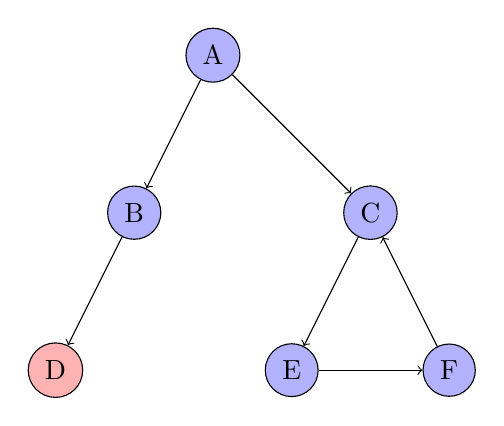
\begin{tikzpicture}
    \node[shape=circle,draw=black, fill = blue!30] (A) at (3,4) {A};
    \node[shape=circle,draw=black, fill = blue!30] (B) at (2,2) {B};
    \node[shape=circle,draw=black, fill = blue!30] (C) at (5,2) {C};
    \node[shape=circle,draw=black, fill = red!30] (D) at (1,0) {D};
    \node[shape=circle,draw=black, fill = blue!30] (E) at (4,0) {E};
    \node[shape=circle,draw=black, fill = blue!30] (F) at (6,0) {F};

    \draw[->] (A) -- (B);
    \draw[->] (A) -- (C);
    \draw[->] (B) -- (D);
    \draw[->] (C) -- (E);
    \draw[->] (E) -- (F);
    \draw[->] (F) -- (C);
  \end{tikzpicture}
  \caption{A graph for depth-first search. The result of $f$ on a vertex and its successors is denoted by the color. Red denotes an error and blue denotes ok.}
  \label{fig:dfsSetProblem}
\end{figure}

\begin{example}
  Suppose we start \dfsstep on the vertex $A$ in the graph depicted in \cref{fig:dfsSetProblem}. Additionally, suppose that the set of visited vertices is $\{B,C,D,E,F\}$. 
  
  As $A$ is not yet visited, we start the exploration process by evaluating $f$ on $A$ and its successors and as seen by the color this evaluates to ok. We have not seen any of the vertices in our walk and therefore call \dfsstep on $B$ and $C$ and it returns ok since $B$ and $C$ are already in the set of visited vertices. Therefore the function in total returns ok for $A$.

  This is however not what we expect it to do. $A$ can reach the vertex $D$ on which $f$ evaluates to an error and it can reach the cycle $[C,E,F,C]$. These wrong evaluations occurred because we assumed in the implementation that the visited set reports this property truthfully. Therefore we require this in every proof. If we run this with an empty set of already visited vertices, then we gain the expected result.
\end{example}

\begin{definition}
  Let $a$ be a vertex in a graph $G$ and \lstinline|f: A → List A → Except String Unit| be a function. We say that $a$ has the \textit{DfsStepSemantics} property if $a$ does not reach a cycle in $G$ and every vertex reachable from $a$ in $G$ evaluates to ok on $f$ with its successors.
\end{definition}

This statement allows us to state the theorem we want to prove for \dfsstep more succinctly.

\begin{theorem}[\dfsstepsematics]\label{trm:dfsstepsematics}
  Let $\vec{v}$ be the input arguments with the vertex $a$ and visited set $V$. If every element in $V$ has the DfsStepSemantics property, then \dfsstep $\vec{v}$ returns ok iff $a$ has the DfsStepSemantics property.
\end{theorem}

\noindent We will prove this statement by induction on the number of vertices not covered by the current walk, i.e. \lstinline|(List.toFinset G.vertices \ List.toFinset currWalk)|, for arbitrary walks and sets of visited vertices. We note that the base case is always true, because if this is equal to zero, then every vertex of $G$ is in the current walk. In $\vec{v}$ we have however explicit proofs that $a$ is a vertex in $G$ and that $a$ is not in the current path, so we have a contradiction. The interesting case is therefore only the induction step. There we need a criteria for when \foldlexceptset returns an error.

In general, this seems hard to do.
Here we already see that the set of visited vertices plays no really important role in the result of the statement as long as all elements in it have the DfsStepSemantics property. As long as we preserve this property in creating the sets we can view \foldlexceptset as individual calls when considering whether it returns an error or not.

\begin{lemma}[\foldlexceptsetisok]\label{lem:foldlexceptsetisok}
  Let $l$ be a list of type $A$ and $S$ be a hash set of type $B$. Consider a property $p: B \to$ \lstinline|Prop| and a function \lstinline|f: A → HashSet B → (Except String (HashSet B))|, that fulfills the following two properties.
  Firstly, that $f$ preserves $p$, i.e. if every element in $S$ has the property $p$ and $f$ returns for the input $a$ and $S$ a set $S'$, then also every element in $S'$ has the property $p$.

  Secondly, that $f$'s acceptance status does not change on sets whose elements fulfill the property $p$, i.e. for any hash sets $S_1, S_2$ such that all elements in each hash set fulfill the property $p$, we have that for any element $a$ $f\ a\ S_1$ returns ok iff $f\ a\ S_2$ returns ok.
  
  Then there exists a hashset $S'$ that \foldlexceptset $f$ $l$ $S$ returns $S'$ iff $f a' S$ returns ok for any element $a'$ in $l$.
\end{lemma}
\begin{proof}
  We prove this by induction on the structure of $l$ for arbitrary $S$.

  If $l$ is empty \foldlexceptset always returns ok and there are no elements in $l$ so that the claim holds.

  If $l$ has the shape $hd::tl$, then $f hd init$ must return a set $S$. If not then \foldlexceptset returns an error and there is an element $a$ from $l=hd::tl$ for which $f a init$ is false so that both sides are false which finishes the proof.

  The result of \foldlexceptset is therefore \lstinline|foldl_except_set f tl S|. From the induction hypothesis, we know that then any element $a$ from $tl$ we have that $f a S$ returns ok iff \foldlexceptset returns ok. We already have the required result for $hd$, it remains to show that always $f\ a\ init$ returns ok. Since $f$ preserves $p$ and any element in $init$ has the property $p$, also any element in $S$ has the property $p$. Therefore we can use the second requirement for $f$ to conclude that  $f\ a\ init$ returns true for any element $a$ from $hd::tl$.
\end{proof}

The property in our case is the DfsStepSemantics property. The first requirement will follow from the induction hypothesis. Therefore it remains to show that \dfsstep preserves the DfsStepSemantics property. 

\begin{lemma}\label{lem:dfsStepProp}[\dfssteppreservesnotReachesCycleAndCounterExample]
  Let $\vec{v}$ be the input arguments with the vertex $a$ and visited set $V$. If every element in $V$ has the DfsStepSemantics property and \dfsstep $\vec{v}$ returns a set $V'$, then every element in $V'$ has the DfsStepSemantics property.
\end{lemma}
\begin{proof}
  We will prove this statement by induction on the number of vertices not covered by the current walk.

  There are two possibilities for \dfsstep to return a set. Firstly, $a$ may be a member of $V$. Then we return $V$ and the claim follows from the assumption.
  Now we consider the possibility of $a$ not being a member of $V$. Then $f$ must return ok for $a$ and its successors and we evaluate the recursive calls on the successors of $a$. By the induction hypothesis, they all return sets with all elements having the DfsStepSemantics property. We can prove by induction on the list, that then also their combination in \foldlexceptset returns a set $V' \setminus \{a\}$ with all elements having the DfsStepSemantics property. Now the claim almost follows but we add the current vertex $a$ into this set. The claim follows as soon as we can show that all successors of $a$ are in $V' \setminus \{a\}$ since none of the successors reach either a cycle or an element where $f$ is evaluated to an error and $f$ is evaluated to ok on the vertex itself. Therefore also $a$ has the DfsStepSemantics property and by that, any element in $V'$ has the property.
\end{proof}

We now want to show that all successors of $a$ are in $V' \setminus \{a\}$. 

\begin{lemma}[\dfsstepreturnsrootelement, \dfsstepsubset]
  Let $\vec{v}$ be the input arguments with the vertex $a$ and visited set $V$. If \dfsstep $\vec{v}$ returns a set $V'$, then $a$ is member of $V'$ and $V \subseteq V'$.
\end{lemma}
\begin{proof}
  We will prove this statement by induction on the number of vertices not covered by the current walk.

  If $a$ is a member of $V$, then we return $V$ and the claim follows as $\subseteq$ is reflexive.
  If $a$ is not a member of $V$, then we return the result of \foldlexceptset on all the successors. Each individual call returns a superset of the input set by the inductive hypothesis. By induction on the size of the list, we see that then also \foldlexceptset returns a superset of $V$ (\foldlexceptsetsubset). In this set, we insert $a$ to obtain $V'$. Therefore it contains $a$ and it is still a superset of $V$.
\end{proof}

Using these results we have a criterion to show when \foldlexceptset contains the original list. Due to Lean internal features, the result must be a bit more technical. As we need to show termination to unfold our function, we call \foldlexceptset not on the successors of $a$ directly, but instead on the attached version of this list, which is a different type. Therefore we talk about the function $g$ in the following result which is supposed to map elements of the subtype \lstinline|{x // x $\in$ G.succesors}| back to the type $A$. 

\begin{lemma}[\foldlexceptsetcontainslistmap]
    Let \texttt{f: A → HashSet B → (Except String (HashSet B))} and {g: A → B} be functions such if $f(a,S) $ returns a hash set $S'$  then $S \subseteq S'$ and $g(a) \in S'$. Then for any list $l$ and hash set S,  if \texttt{foldl\_except\_set f l S} returns a hash set $S'$, then for all elements $a$ of $l$, $g(a) \in l$.
\end{lemma}
\begin{proof}
    We prove this by induction on $l$.
    If $l$ is empty all elements of $l$ are in their mapped form in the resulting set.

    If $l$ has the shape $hd::tl$, then we first compute $f(hd,S)$ which must return a set $S'$ since the whole function returns a set. $S'$ must contain $g(hd)$ and is passed into \texttt{foldl\_except\_set} which by the induction hypothesis contains all elements of $tl$ in their mapped form. Due to the subset property, all elements of $S'$ must also be contained, so that also $g(hd)$ is in the result. Therefore all elements of the list are contained in their mapped form in the resulting set, if it exists.
\end{proof}

Now we know that all successors of $a$ are in $V'\setminus\{a\}$ and we finish the claim in \cref{lem:dfsStepProp}. This also finishes the preparations to prove \cref{trm:dfsstepsematics}.

\begin{proof}[Proof of \cref{trm:dfsstepsematics}]
  We prove this by induction on the number of uncovered vertices i.e. vertices that are in $G$, but not in the current walk. The base case is trivial as it contradicts the inputs \dfsstep.

  In the induction step, we prove both directions separately. In the forward direction \dfsstep returns a set $V'$ and we want to show that $a$ has the DfsStepSemantics property. We know that every element in  $V'$ has the DfsStepSemantics property and that $a$ is in $V'$. Hence, the forward direction is proven.

  In the backward direction, we know that $a$ has the DfsStepSemantics property and want to show that \dfsstep returns ok. If $a$ is in $V$, then we return ok and the claim is proven. Now assume that $a$ is not in $V$. Since $a$ has the DfsStepSemantics property and $a$ can reach itself $f$ must be evaluated to ok on $a$ and its successors. Additionally, none of the successors of $a$ can occur in the current path as this would imply that $a$ can reach a cycle. 
  It remains to show that \foldlexceptset returns ok for which we use \cref{lem:foldlexceptsetisok}. We know that \dfsstep returns a superset of the input set \cref{lem:dfsStepProp} and by the induction hypothesis all individual calls are ok iff the vertex has the DfsStepSemantics property which marks the independence of the visited set. We only have to show that all successors of $a$ have the DfsStepSemantics property and use the induction hypothesis to show the claim. This follows due to the propagating properties of the DfsStepSemantics property. If any successor of $a$ reaches a cycle, then also $a$ would reach a cycle, which we know is not true. Similarly, any element reachable from a successor of $a$ is also reachable from $a$ and therefore has to evaluate to ok with its successor.
\end{proof}

Now we can show the proof of \cref{trm:dfssemantics}.

\begin{proof}[Proof of \cref{trm:dfssemantics}]
  As \dfs is only the repeated evaluation of \dfsstep wrapped in \foldlexceptset, we again employ \cref{lem:foldlexceptsetisok} to reduce it to individual calls and use \cref{lem:dfsStepProp} and \cref{trm:dfsstepsematics} to fulfill the requirements as in the previous proof. 

  Therefore we only have to show that all vertices have the DfsStepSemantics property iff the graph is acyclic and every vertex of the graph is evaluated to ok on $f$ with its successors which we have already shown in \cref{lem:acyclicIffAllNotReachCycle} and \cref{lem:allTrueIfAllCanReachTrue}
\end{proof}


\section{HashSets for depth-first search}

In the previous section, we implement and prove the correctness of our depth-first search implementation. The proofs are independent of the underlying set implementation and also work with finite sets which we used first. A faster implementation is possible by using hash-based data structures such as hash maps and hash sets. Unfortunately, hash maps and hash sets almost have no lemmas proven about them already in Mathlib. Finite sets have in contrast already have many results proven about them. We try to bridge the gap by showing some results about the correctness of operations and presenting which assumptions we use as axioms. As the main focus of the thesis is not to formally verify hash sets we will only give a general overview of our results.

Hash maps are defined in Lean's standard library. We define hash sets as a hashmap mapping elements to the unit type. This will allow us to reuse the results we prove for hash sets in the hash map case which was our underlying graph model.

\begin{lstlisting}
  abbrev HashSet (A:Type) [Hashable A] [DecidableEq A] := HashMap A Unit
\end{lstlisting}

A hash map consists of buckets that are implemented as associative lists, which are essentially lists of pairs. The buckets are stored in a non-empty array.

\begin{lstlisting}
  def Std.HashMap.Imp.Buckets (α : Type u) (β : Type v) := {b : Array (AssocList α β) // 0 < b.size}
\end{lstlisting}

The hash map implementation combines the buckets with the size property as a natural number to see when the hash map has to be resized as very large buckets decrease the advantages in speed. 

\begin{lstlisting}
structure Std.HashMap.Imp (α : Type u) (β : Type v) where
  size    : Nat
  buckets : Imp.Buckets α β
\end{lstlisting}

This is so far only a reorganization of the data and does not explain the advantages. Indeed, placing elements randomly in buckets is not effective. The important property is called the well-formedness of the hash map buckets in Lean. This requires the underlying type to be hashable, i.e. a hash function for this type exists, and to have a boolean equality (\lstinline|BEq|) which is a user-defined equality in contrast to the real equality based on the type. We do not care in this work about the boolean equality and use the equality of the type directly.

The well-formedness of a hash map bucket consists of two properties. Firstly, in every bucket, every element occurs at most once so that after an update no old values remain. Secondly, any element is only the bucket whose position in the array equals the hash value modulo the size. This allows us to only check a small part of the array. The hash map implementation is well-formed if the buckets are well-formed and the size property matches the number of buckets.

\begin{lstlisting}
structure Std.HashMap.Imp.Buckets.WF [BEq α] [Hashable α] (buckets : Buckets α β) : Prop where
  distinct [LawfulHashable α] [PartialEquivBEq α] : ∀ bucket ∈ buckets.1.data,
    bucket.toList.Pairwise fun a b => ¬(a.1 == b.1)
  hash_self (i : Nat) (h : i < buckets.1.size) :
    buckets.1[i].All fun k _ => ((hash k).toUSize % buckets.1.size).toNat = i
\end{lstlisting}

A hash map is then finally a well-formed hash map implementation. The hash map is mostly a wrapper around the hash map implementation and therefore we focus in this section on the proofs on the \lstinline|Std.HashMap.Imp| level.

\begin{lstlisting}
  def Std.HashMap (α : Type u) (β : Type v) [BEq α] [Hashable α] := {m : Imp α β // m.WF}
\end{lstlisting}

The contains function uses the well-formedness of the hash map implementation to look in the bucket placed in the position of the hash value of the element. The function \lstinline|mkIdx| calculates the position and provides a proof that there is a bucket at this position.

\begin{lstlisting}
def contains [BEq α] [Hashable α] (m : Imp α β) (a : α) : Bool :=
  let ⟨_, buckets⟩ := m
  let ⟨i, h⟩ := mkIdx buckets.2 (hash a |>.toUSize)
  buckets.1[i].contains a
\end{lstlisting}

In the depth-first search implementation, we only need the insertion and contains function as we only add the visited vertices. We never unvisit an element and therefore focus on the insertion function. We are given two elements $a$ and $b$. If $a$ is already present in the bucket of its hash value we simply replace the old value of $a$ by $b$ in $a$'s bucket. If $a$ is not present we add the element at the front of the corresponding bucket. This might increase the size to a value that is larger than the capacity. In this case, expand creates a new larger empty bucket and reinserts all the previous elements.

\begin{lstlisting}
def insert [BEq α] [Hashable α] (m : Imp α β) (a : α) (b : β) : Imp α β :=
  let ⟨size, buckets⟩ := m
  let ⟨i, h⟩ := mkIdx buckets.2 (hash a |>.toUSize)
  let bkt := buckets.1[i]
  bif bkt.contains a then
    ⟨size, buckets.update i (bkt.replace a b) h⟩
  else
    let size' := size + 1
    let buckets' := buckets.update i ( AssocList.cons a b bkt) h

    if numBucketsForCapacity size' ≤ buckets.1.size then
      { size := size', buckets := buckets' }
    else
      expand size' buckets'
\end{lstlisting}

The main result we want to prove is concerned with the correctness of the insertion with regard to the contains function.

\begin{lemma}[\StdHashSetcontainsinsert]
  Let $S$ be a hash set and $a$ an element. For any element $a'$, $a'$ is contained in the insertion of $a$ into $S$ iff $a'$ is contained in $S$ or $a'$ and $a$ are equal.
\end{lemma}

As hash maps are not only used to serve as hash sets but also as the graph model we want a more general result to reuse. The contains function does not tell us something about the value that is contained with the key. In order to reason about the key-value pairs we introduce the key-value member \lstinline|kv_member| which is true whenever a key-value pair is in the bucket corresponding to the key.

\begin{lstlisting}
  def (.\StdHashMapImpkvmember.) (m: HashMap.Imp A B) (a: A) (b:B): Bool :=
    let ⟨_, buckets⟩ := m
    let ⟨i, h⟩ := mkIdx buckets.2 (hash a |>.toUSize)
    let bkt := buckets.1[i]

    (a,b) ∈ bkt.toList
\end{lstlisting}

An element $a$ is contained in $m$ iff there exists an element $b$ with $a$ and $b$ being a \StdHashMapImpkvmember as we look in the same bucket in both cases. Both functions use however the mkIdx function to access the elements. As we are only using hash maps, we can consider any well-formed hash map implementations and collect all elements in the buckets in a single finite set, the key-value set \StdHashMapImpkv.

\begin{lstlisting}
  def (.\StdHashMapImpBucketskv.) (buckets: HashMap.Imp.Buckets A B): Finset (A × B) := Array.foldl (fun x y => x ∪ y.toList.toFinset) ∅ buckets.val

  def (.\StdHashMapImpkv.) (m: HashMap.Imp A B): Finset (A × B) := m.2.kv
\end{lstlisting}

By induction on the size of the list, we manage to show that an element is in \StdHashMapImpkv iff it is in some bucket given as an input to (\StdArrayfoldlunion). Additionally, we  
show that \StdHashMapImpkv is equivalent to \StdHashMapImpkvmember.

\begin{lemma}[\StdHashMapImpkvmemberiffinkv]
  Let $m$ be a well-formed hash map implementation. Then for any elements $a$ and $b$, $a$ and $b$ are a key-value member of $m$ iff $a$ and $b$ are in $m.kv$.
\end{lemma}
\begin{proof}
  Any $a$ and $b$ that are a key-value member of $m$ are in a bucket and hence in $m.kv$. For the reverse direction, we need the well-formedness. If $a$ and $b$ are in $m.kv$, they are in some bucket $bkt$ of $m$. Due to the well-formedness of $m$, this bucket is accessible by the hash value of $a$. Therefore $a$ and $b$ are also a key-value member of $m$.
\end{proof}

In the following proof for the insertion, we can therefore use the key-value set and do not have to use the more complicated functions using the hash-value.

\begin{lemma}[\StdHashMapImpinsertsemantics]
  Let $m$ be a well-formed hash map implementation. Then for any keys $a$ and $a'$ and values $b$ and $b'$, we have that $a'$ and $b'$ are a key-value member of $m.insert a b$ iff $a'$ and $b'$ are a key-value member of $m$ and $a$ and $a'$ are different, or if $(a,b)$ and $(a',b')$ are equal.
\end{lemma}
\begin{proof}
The first two cases are rather obvious as we only change a single bucket. If $a$ is already contained in $m$, we replace its value by $b$. Hence all key-value members of this hash map implementation are all the previous members of $m$ except for the replaced previous value for $a$ or the new pair $(a,b)$. The second case is where $a$ is not contained in $m$ and adding the new pair does not bring the hash map implementation over its maximum size. In this case, we add the element to the front of the bucket. All previous key-value members are preserved and as $a$ is not contained, there is no other pair with the key $a$, so the claim follows.

In the last case, adding $(a,b)$ brings the hash map implementation over its maximum size. Hence a larger hash map implementation is created and every element reinserted. Until then we added $(a,b)$ as in the previous case so that it only remains to show that all key-value members are preserved which we show by showing that the key-value set is equal (\StdHashMapImpexpandpreservesmem). The main work of this proof is done in \StdHashMapImpexpandgomem by induction but is rather low-level and hence omitted here.
\end{proof}

This result is the main result of this section and we will use it to now formally verify the real operations that we use in the program. As the hash map is a pair of the implementation and a proof of the implementation's well-formedness, we can lift these results to hash maps as desired. We already noted that $a$ is contained in a hash map $m$ iff there exists a $b$ such that $a$ and $b$ are a key-value member of $m$. Hence we gain the desired result for the contains function.

\begin{lemma}[\StdHashMapcontainsinsert]
  Let $m$ be a hash map. Then for any elements $a$ and $a'$ and $b$, $a'$ is contained in $m.insert a b$ iff $a'$ is contained in $m$ or $a$ and $a'$ are equal.
\end{lemma}

A hash set of type $A$ was defined as a hash map mapping elements of type $A$ to the unit type. Hence, the result for hash sets follows as well.

\begin{lemma}[\StdHashSetcontainsinsert]
  Let $S$ be a hash set and $a$ an element. For any element $a'$, $a'$ is contained in the insertion of $a$ into $S$ iff $a'$ is contained in $S$ or $a'$ and $a$ are equal.
\end{lemma}

We additionally use the \lstinline|findD| function to look up values for a key $a$. This function uses \lstinline|find?| to look for a key $a$ which returns an option. If this option contains an element it is returned else we return the given default element.

\begin{lstlisting}
def find? [BEq α] [Hashable α] (m : Imp α β) (a : α) : Option β :=
  let ⟨_, buckets⟩ := m
  let ⟨i, h⟩ := mkIdx buckets.2 (hash a |>.toUSize)
  buckets.1[i].find? a

def findD (self : HashMap α β) (a : α) (b₀ : β) : β := (self.find? a).getD b₀
\end{lstlisting}

An alternative characterization of findD that simplifies our later work is the following.

\begin{lstlisting}
  lemma (.\StdHashMapfindDeqfind.) (m: HashMap A B) (a:A) (b:B): m.findD a b = match m.find? a with
                    | some b' => b'
                    | none => b
\end{lstlisting}

In a well-formed hash-map implementation $m$, $b$ is the result of $m.find?\ a$ iff $a$ and $b$ are key-value members of $m$ as we look in the same bucket and every element in a well-formed bucket has a unique key. (\StdHashMapfindiffkv) Therefore we can reuse the insertion semantics in the $find?$ case:

\begin{lemma}[\StdHashMapfindinsert]\label{lem:hmfindinsert}
  Let $m$ be a hash map and $a$ and $b$ be a key-value pair. Then for any element $a'$, \lstinline|(m.insert a b).find? a'| yields \lstinline|some b| iff $a$ and $a'$ are equal or else the result of $m.find?\ a'$.
\end{lemma}

In the graph, we never use $find?$ as we do not want to deal with the option type. We instead use $findD$ and use the empty list as the default element. One requirement would be that the result of $findD$ is correct for any key $a$ after inserting $a$ with a value $b$.

\begin{lemma}[\StdHashMapfindDinserttwo]
  Let $m$ be a hash map and $a$ and $b$ be a key-value pair. For any elements $b'$,\lstinline|(m.insert a b).findD a b'| yields $b$.
\end{lemma}
\begin{proof}
  By \cref{lem:hmfindinsert} \lstinline|(m.insert a b).find? a| yields \lstinline|some b|. By the definition of \lstinline|findD|, therefore \lstinline|findD| also returns $b$ and the claim is proven.
\end{proof}

The operations \lstinline|contains| and \lstinline|findD| are sufficiently verified for our purposes. These results can also be reused as long as the used equality is the equality of the type and not a user-defined \lstinline|BEq|.

We did not manage to verify the \lstinline|ofList| operation that takes a list $l$ of pairs of the type $A \times B$ and converts it into a \lstinline|HashMap A B| $m$. We use it to create the initial graph and desire that the result of findD is the same on $l$ and $m$ so that the graph is exactly the given input (\StdHashMapfindDofListislistfindgetD). 